\documentclass[11pt]{article}
\usepackage[margin=1in]{geometry}
\usepackage{amsmath,amssymb,amsthm,mathtools}
\usepackage{graphicx,booktabs,microtype,xcolor,enumitem}
\usepackage[numbers,sort&compress]{natbib}
\usepackage[colorlinks=true,linkcolor=blue!50!black,citecolor=blue!50!black,urlcolor=blue!50!black]{hyperref}
\usepackage{listings}
\lstset{basicstyle=\ttfamily\small,columns=fullflexible,frame=single,framerule=0.3pt,xleftmargin=4pt,xrightmargin=4pt}

\newtheorem{theorem}{Theorem}
\newtheorem{proposition}[theorem]{Proposition}
\newtheorem{corollary}[theorem]{Corollary}
\newtheorem{lemma}[theorem]{Lemma}
\theoremstyle{definition}
\newtheorem{definition}{Definition}
\theoremstyle{remark}
\newtheorem{remark}{Remark}

\newcommand{\E}{\mathbb{E}}
\newcommand{\Prob}{\mathbb{P}}
\newcommand{\SR}{\widehat{\mathrm{SR}}}
\newcommand{\tH}{t_{H}}
\newcommand{\cT}{\mathcal{T}}

\title{Deflate by Bits, Not Trials:\\Why Query-Counted Deflated Sharpe Ratios Fail Under Adaptive Search,\\and a Sealed-Holdout Remedy}
\author{Shlok Sobti\\Invsify Technologies\\\texttt{shlok@invsify.com}}
\date{October 2026}

\begin{document}
\maketitle

\begin{abstract}
The Deflated Sharpe Ratio (DSR) is the standard defence against backtest overfitting. It raises the significance bar with the \emph{number} of strategies tried, and recent work proposes logging every trial so that DSR can be applied to the true search intensity. We show that counting the backtests actually run is the wrong currency whenever the researcher is \emph{adaptive}, that is, whenever each new strategy is chosen after seeing earlier validation results. This describes everyday quantitative practice, and it describes LLM research agents and RL alpha miners by construction.

First, we prove that a one-line ``combine what worked'' procedure over $k$ pure-noise strategies drives the validation $t$-statistic to $\sqrt{2k/\pi}\,(1+o_p(1))$, independently of cross-strategy correlation. The DSR bar for the same complete ledger grows only as $\sqrt{2\ln k}$, so DSR certifies noise with probability tending to one. Second, we prove a matching positive result. If the holdout can reveal only a transcript from a set $\cT$, then certifying at $t>\bar G^{-1}(\alpha/|\cT|)$ is valid for \emph{every} adaptive analyst. DSR is the non-adaptive special case $|\cT|=N$, and overfitting scales as $\Theta(\sqrt{\text{bits revealed}})$ rather than $\sqrt{\ln(\text{queries})}$. Under full-precision Sharpe feedback, the only generic valid correction is the classical span (Scheff\'e/GRS) bound, which grows as $\sqrt{\dim}$ and is unusable at realistic scale. This motivates a \emph{sealed holdout}: an opaque type whose only operation is a budgeted PASS/FAIL verdict.

On synthetic markets, and on 423 real industry strategies (1970--2026) under a stationary-bootstrap null, ordinary adaptive workflows such as ``rank on validation, keep the top $j$'' are certified by complete-ledger DSR on 84--100\% of pure-noise replicates. Sealed-verdict variants hold false certification at 0.8--3.0\%. It matches the power of a one-shot holdout when the signal regime is stable, but, like any train-then-test protocol, it loses power when the regime rotates. We also place open-weight LLM agents (7B and 72B) and GRPO-trained miners in the loop. They exhibit the combine-the-winners behaviour and inflate validation Sharpe, but at current scale they search too inefficiently to cross the DSR bar (2 of 72 null episodes certified). We therefore present them as an emerging risk rather than a demonstrated failure.
\end{abstract}

%======================================================================
\section{Introduction}
%======================================================================
A backtest is a hypothesis test whose researcher can see the answer key. Finance has long known that searching over many strategies and reporting the best manufactures significance \citep{lo1990data,sullivan1999data,white2000reality,harvey2016cross}. The modern standard remedy is to \emph{count the search}. The Deflated Sharpe Ratio \citep{bailey2014deflated} raises the significance bar with the number of trials $N$, roughly as $\sqrt{2\ln N}$ standard errors. The Probability of Backtest Overfitting \citep{bailey2017pbo} and reality-check bootstraps \citep{white2000reality,hansen2005spa,romano2005stepwise} likewise treat the search as a fixed family of candidates.

Real research is not a fixed family. A researcher who sees that momentum in banks and in insurers both validated well will try them together next; one who sees a signal fail will flip or drop it. Each step is innocuous, yet the candidate list is being written \emph{by} the validation set. The question is acute now that this loop is being automated. LLM agents read a backtest and write the next hypothesis, and RL miners optimise a validation metric directly \citep{yu2023alphagen,shi2025alphaforge}. Two recent responses illustrate the state of the art. \citet{gencay2026honest} give an LLM discovery system a complete \emph{trial ledger} so that DSR can be indexed to the true search intensity. \citet{qu2026propose} score factors only on post-submission (live) data with anytime-valid e-processes, paying roughly 500 trading days of waiting per verdict. The first assumes that counting trials suffices for historical backtests. The second gives up on historical backtests.

\paragraph{This paper.} We show that for adaptive researchers the right currency is \emph{information}, not trials. We make this precise for Sharpe-ratio certification and test it empirically.
\begin{enumerate}[leftmargin=*,itemsep=2pt]
\item \textbf{Complete-ledger DSR is invalid under adaptive search (Theorem~\ref{thm:attack}, Corollary~\ref{cor:dsr}).} An analyst who queries $k$ pure-noise strategies, goes long the above-median ones and short the rest obtains a validation $t$-statistic of $\sqrt{2k/\pi}(1+o_p(1))$ for any common correlation. DSR fed the complete $(k{+}1)$-trial ledger certifies it with probability $\to1$. Empirically, the everyday ``keep the top-$j$ by validation Sharpe'' workflow is DSR-certified on 95\% of synthetic and 84\% of real-data null replicates, and greedy combination on 97--100\%.
\item \textbf{Information budgets give valid certificates (Theorem~\ref{thm:transcript}).} If everything the analyst can learn about the holdout is a transcript from a set $\cT$, the bar $\bar G^{-1}(\alpha/|\cT|)$ controls false certification for \emph{any} analyst, however adaptive. DSR's $\sqrt{2\ln N}$ is the special case of $\ln N$ nats. The $\sqrt{\text{bits}}$ rate is attained up to constants (Proposition~\ref{prop:tight}), and with full-precision feedback the only generic alternative is the classical span bound, which pays $\sqrt{\dim}$ (Proposition~\ref{prop:span}).
\item \textbf{A sealed holdout (Section~\ref{sec:sealed}).} We turn the theory into an interface: the holdout is an opaque type whose only eliminator is \texttt{verdict(strategy) -> PASS|FAIL}, with a query budget $K$ and a fixed bar $\bar G^{-1}(\alpha/K)$. Validity holds by construction for any proposer, human, scripted, LLM or RL, without trusting or even logging it.
\item \textbf{Evidence (Section~\ref{sec:exp}).} We give theory-matching simulations (E1); a validity and power study including regime rotation (E2); 423 real hedged industry strategies with a stationary-bootstrap null (E3); and two exploratory studies of automated researchers, open-weight LLM agents (E4) and GRPO alpha miners (E5). The automated researchers reproduce the attack's \emph{behaviour} but realise only a fraction of its \emph{capacity}. We report this as a measured gap, not as a failure of DSR.
\end{enumerate}

\paragraph{What is and is not new.} Adaptive data analysis is a mature area of theoretical computer science and statistics \citep{dwork2015science,dwork2015generalization,hardt2014preventing,bassily2016algorithmic,russo2016controlling,xu2017information}. Our attack is a Sharpe-ratio relative of Freedman's paradox \citep{freedman1983note} and of the boosting attack on ML leaderboards \citep{blum2015ladder}. Theorem~\ref{thm:transcript} is a high-probability transcript-counting bound in the spirit of description-length arguments \citep{dwork2015generalization} and mutual-information bounds \citep{russo2016controlling}. Span bounds for the maximum Sharpe ratio are classical \citep{scheffe1953method,gibbons1989test}. Our contributions are (i) to show, formally and on real data, that the instrument now proposed for automated research, query-counted ledger DSR, fails under adaptive search; (ii) to identify DSR as the $\ln N$-nat special case of an information-budget certificate, which yields a drop-in valid replacement; (iii) to package that replacement as a typed interface that automated researchers can be given safely; and (iv) to measure how far current LLM and RL researchers are from exploiting the gap. To our knowledge (i)--(iv) have not appeared in the finance or LLM-agent literature.

%======================================================================
\section{Setup}
%======================================================================
A holdout $H=(r_t)_{t=1}^n$ consists of $n$ periods of returns on $k$ base strategies, $r_t\in\mathbb R^k$. A strategy is a weight vector $w\in\mathbb R^k$ with return series $w^\top r_t$, per-period Sharpe ratio $\SR_H(w)=\bar x/s_x$, and $t$-statistic $\tH(w)=\sqrt n\,\SR_H(w)$.

\paragraph{Null.} Under $H_0$ the rows $r_t$ are i.i.d.\ with mean zero. For any $w$ chosen independently of $H$, $\tH(w)$ is exactly Student-$t_{n-1}$ for Gaussian rows and asymptotically standard normal in general. Write $\bar G(c)=\Prob(t_{n-1}>c)$.

\paragraph{Analysts and channels.} An analyst (human, LLM agent or RL policy) interacts with $H$ only through a \emph{channel}. On the $j$-th query $w_j$ the channel returns an answer $a_j$, and the transcript is $\pi=(a_1,a_2,\dots)$. Everything else the analyst uses is collected into $U$: training data, model weights, prompts, sampling randomness. We assume $U$ is independent of $H$. The analyst reports $\hat w=f(U,\pi)$ and the holdout \emph{certifies} it if $\tH(\hat w)$ exceeds a bar. Validity means $\Prob_{H_0}(\text{certify})\le\alpha$. The status-quo channel returns $a_j=\SR_H(w_j)$ in full precision.

\paragraph{DSR on a ledger.} Given a ledger of $N$ trials whose holdout Sharpe estimates have cross-sectional variance $V$, DSR \citep{bailey2014deflated} is
\begin{equation}\label{eq:dsr}
\mathrm{DSR}=\Phi\!\left(\frac{(\SR-\SR_0)\sqrt{n-1}}{\sqrt{1-\hat\gamma_3\SR+\tfrac{\hat\gamma_4-1}{4}\SR^2}}\right),\qquad
\SR_0=\sqrt V\Big[(1-\gamma)\Phi^{-1}(1-\tfrac1N)+\gamma\Phi^{-1}(1-\tfrac1{Ne})\Big],
\end{equation}
with $\gamma$ the Euler--Mascheroni constant. A strategy is certified when $\mathrm{DSR}>0.95$. The bracket approximates $\E\max$ of $N$ i.i.d.\ standard normals, $\approx\sqrt{2\ln N}$.

%======================================================================
\section{Theory}
%======================================================================
\subsection{Query counting fails under adaptivity}

\begin{theorem}[Adaptive ensemble attack]\label{thm:attack}
Let the rows of $H$ be i.i.d.\ $\mathcal N(0,\Sigma)$ with $\Sigma=(1-\rho)I_k+\rho\mathbf 1\mathbf 1^\top$, $\rho\in[0,1)$, and $k$ even. The analyst queries each base strategy once, observes $Z_i=\tH(e_i)$, and reports
\[\hat w=\tfrac1k s,\qquad s_i=\operatorname{sign}\big(Z_i-\operatorname{med}(Z)\big)\quad\text{(rank long--short)}.\]
Then for fixed $k$, as $n\to\infty$, $\tH(\hat w)\Rightarrow k^{-1/2}\sum_{i=1}^k|\varepsilon_i-\operatorname{med}(\varepsilon)|$ with $\varepsilon\sim\mathcal N(0,I_k)$, and consequently
\[\frac{\tH(\hat w)}{\sqrt{2k/\pi}}\;\longrightarrow\;1\quad\text{as }k\to\infty\text{ (after }n\to\infty),\qquad\text{independently of }\rho.\]
For $\rho=0$ the sign-flip portfolio $s_i=\operatorname{sign}(Z_i)$ has the same limit, and the keep-winners portfolio ($s_i=\mathbf{1}\{Z_i>0\}$, normalised) has limit $\sqrt{k/\pi}$.
\end{theorem}
\begin{proof}[Proof sketch]
Write the asymptotic joint law $Z=\sqrt\rho F\mathbf 1+\sqrt{1-\rho}\,\varepsilon$. Subtracting the median removes $F$, so $s$ depends only on $\varepsilon$, and $\mathbf 1^\top s=0$ removes the factor from the portfolio. The portfolio's mean is $\sqrt{1-\rho}\sum_i|\varepsilon_i-\operatorname{med}\varepsilon|/(k\sqrt n)$ and its variance is $s^\top\Sigma s/k^2=(1-\rho)/k$. Selection perturbs the sample variance only at $O_p(n^{-1/2})$. Hence $\tH(\hat w)\to k^{-1/2}\sum_i|\varepsilon_i-\operatorname{med}\varepsilon|$. Since the median of $\varepsilon$ tends to $0$ and $\E|\varepsilon_1|=\sqrt{2/\pi}$, the law of large numbers gives the ratio limit. Appendix~\ref{app:proofs} gives the details.
\end{proof}

The attack needs no cleverness. It is the procedure ``keep what worked, short what didn't, stay market-neutral'' that an LLM agent or a junior quant performs unprompted. Its validation $t$ grows like $\sqrt k$, whereas any correction indexed by the number of \emph{queries} grows like $\sqrt{\ln k}$. The limits are sequential ($n\to\infty$ first). E1 shows that the approximation is already accurate at $k/n\approx0.4$ (25.21 against 25.23 at $k=1000$, $n=2520$).

\begin{corollary}[Query-counted ledger DSR certifies noise]\label{cor:dsr}
Under the conditions of Theorem~\ref{thm:attack}, let the ledger record all $N=k+1$ trials, the $k$ base strategies plus $\hat w$. Then $nV\to(1-\rho)+2/\pi+o(1)$ and the DSR $z$-score is at least $\sqrt{2k/\pi}-c_\rho\sqrt{2\ln(k+1)}\to\infty$, with $c_\rho\le\sqrt{1+2/\pi}(1+o(1))$. Hence $\Prob_{H_0}(\mathrm{DSR}>1-\alpha)\to1$ for every $\alpha>0$. (We use that the bracket in~\eqref{eq:dsr} is at most $\sqrt{2\ln N}$, which we verified numerically for $2\le N\le10^7$, where the ratio is at most $0.935$.)
\end{corollary}

At $k=50$, already typical of a short agent session, the attack's expected $t$ is $5.6$, while the validation $t$ that DSR requires for certification is about $4.6$; at $k=1000$ the numbers are $25.2$ versus $5.8$. In E1, ledger DSR certifies the rank long--short attack with probability $1.00$ from $k=50$ and keep-winners from $k=100$ ($\rho=0$), and greedy forward selection with probability $\ge0.95$ from $k=100$ ($\rho=0$) or $k=200$ ($\rho>0$).

\paragraph{What ``trials'' should mean.} \citet{bailey2014deflated} intend $N$ to count the effectively independent configurations \emph{considered}, not the backtests \emph{run}. The sign attack implicitly considers all $2^k$ sign patterns, and DSR with $N=2^k$ gives a bar of about $\sqrt{2k\ln2}$, which is valid. Our target is therefore \emph{query-counted} DSR, where $N$ is read from a ledger of backtests run, as in current LLM-discovery systems \citep{gencay2026honest} and in most practice. The difficulty is that for an adaptive researcher the set of configurations implicitly considered is not observable from the ledger. Section~\ref{sec:bits} makes it observable by fixing it in the channel.

\subsection{Deflate by bits: a certificate valid for any analyst}\label{sec:bits}

\begin{theorem}[Transcript certificate]\label{thm:transcript}
Let $\cT$ be a countable set containing every transcript the channel can produce, and let $q$ be a probability mass function on $\cT$ fixed before the analysis. For any analyst with $U$ independent of $H$, under $H_0$,
\[\Prob\Big(\tH(\hat w)>\bar G^{-1}\big(\alpha\,q(\pi)\big)\Big)\le\alpha.\]
In particular, with $|\cT|<\infty$ and $q$ uniform, certifying at $c_\cT=\bar G^{-1}(\alpha/|\cT|)\approx\sqrt{2\ln(|\cT|/\alpha)}$ is valid. The statement is exact for Gaussian rows. For non-Gaussian rows it holds asymptotically provided $\alpha/|\cT|$ stays within the moderate-deviation range of the self-normalised $t$-statistic (for example a finite third moment and $c_\cT=o(n^{1/6})$).
\end{theorem}
\begin{proof}
For each $\tau\in\cT$ let $\hat w_\tau=f(U,\tau)$ be what the analyst would report had it seen $\tau$. Conditional on $U$, $\hat w_\tau$ is fixed and independent of $H$, so $\Prob(\tH(\hat w_\tau)>\bar G^{-1}(\alpha q(\tau))\mid U)\le\alpha q(\tau)$. The realised report is $\hat w_\pi$, so the bad event is contained in $\bigcup_\tau\{\tH(\hat w_\tau)>\bar G^{-1}(\alpha q(\tau))\}$. A union bound gives $\sum_\tau\alpha q(\tau)=\alpha$.
\end{proof}

The bar depends only on how much the channel \emph{can} reveal, $\ln|\cT|$ nats (or the code length $-\ln q(\pi)$). It does not depend on the analyst, on how many trials it ran, or on whether its ledger is honest.

\begin{corollary}[Instances]\label{cor:instances}
\begin{enumerate}[label=(\roman*),leftmargin=*,itemsep=1pt]
\item \emph{Pre-registered best-of-$N$.} If the report depends on the holdout only through $\arg\max_j\tH(w_j)$ over $N$ fixed candidates, then $|\cT|=N$ and $c=\bar G^{-1}(\alpha/N)\approx\sqrt{2\ln N}$. This is the Bonferroni form of the DSR bar. DSR replaces the quantile by an expected maximum and estimates the scale $\sqrt V$ from the ledger. That makes it a heuristic rather than a level-$\alpha$ test even without adaptivity: when trials are highly correlated, $nV\ll1$ shrinks the bar (E4 shows null certifications driven by $nV\approx0.1$--$0.4$).
\item \emph{Sealed verdict.} The channel answers PASS iff $\tH(w_j)>c$, allows at most $K$ queries and stops at the first PASS. Along the all-FAIL path every query is a fixed function of $U$, so a false PASS requires one of $K$ fixed strategies to exceed $c$, and $c_K=\bar G^{-1}(\alpha/K)$ is valid. In our experiments we use the slightly conservative $\bar G^{-1}(\alpha/(K+1))$.
\item \emph{Ladder with budget $B$} \citep{blum2015ladder}. If at most $B$ of $m$ answers are positive bits, then $|\cT|\le\sum_{b\le B}\binom mb$.
\item \emph{Full-precision feedback.} $\cT$ is uncountable and Theorem~\ref{thm:transcript} is vacuous. Proposition~\ref{prop:span} below gives the only generic alternative.
\end{enumerate}
\end{corollary}

\begin{proposition}[Span bound; Scheff\'e, Gibbons--Ross--Shanken]\label{prop:span}
If every report lies in the span of $k$ fixed base strategies, then under Gaussian $H_0$, $\max_{w}\tH(w)^2=n\,\bar r^\top\hat\Sigma^{-1}\bar r\sim\frac{k(n-1)}{n-k}F_{k,n-k}$ \citep{scheffe1953method,gibbons1989test}. Certifying at $c_{\mathrm{span}}=\big(\frac{k(n-1)}{n-k}F^{-1}_{k,n-k}(1-\alpha)\big)^{1/2}\approx\sqrt k$ is therefore valid for \emph{any} analyst and \emph{any} feedback precision.
\end{proposition}

So full-precision feedback can be corrected, but only by paying for the dimension of the strategy space rather than the number of queries. The bar is $8.3$ for $k=50$ and $23.4$ for our $k=423$ real strategies, so it certifies essentially nothing (E2, E3), and it is undefined when the strategy space is unrestricted, as for code-writing agents. The attack of Theorem~\ref{thm:attack} attains $0.80$ of it.

\begin{proposition}[The $\sqrt{\text{bits}}$ rate is attained]\label{prop:tight}
A channel revealing $b$ bits admits the valid bar $\bar G^{-1}(\alpha2^{-b})=\sqrt{2b\ln2}\,(1+o(1))\approx1.18\sqrt b$. The sign-flip attack of Theorem~\ref{thm:attack} uses exactly $b=k$ bits, namely $\operatorname{sign}(Z_i)$, and achieves $\sqrt{2b/\pi}\approx0.80\sqrt b$. For $b=o(n)$ bits, the worst-case validation inflation is therefore $\Theta(\sqrt b)$, within the constants $0.80$ and $1.18$, and DSR's $\sqrt{2\ln N}$ is the $b=\log_2N$ instance. When $b\gtrsim k$ the span bound is the tighter of the two. The bits bound is useful precisely when $b\ll k$, which is what a sealed channel enforces.
\end{proposition}

The practical message is that a holdout should be accounted for by what it \emph{says}, not by what it is asked. A verdict-only holdout queried $K=30$ times reveals at most $\log_2 31\approx5$ bits, and its bar ($t>2.94$ at $\alpha=0.05$) is \emph{lower} than the $t\approx3.7$ that DSR demands of the best of 30 pre-registered trials. A holdout that prints annualised Sharpe ratios in $[-3,3]$ to two decimals for 30 queries reveals up to $30\log_2600\approx277$ bits, so the bits bar is $t\approx19.7$, and the alternative span bar is $23.4$ for our universe. Both are useless.

%======================================================================
\section{The sealed holdout as a typed primitive}\label{sec:sealed}
%======================================================================
Theorem~\ref{thm:transcript} moves validity from the analyst's behaviour, which we cannot audit for an LLM or an RL policy, into the \emph{type} of the holdout, which we can enforce. The interface below is complete: there is no accessor that returns data, scores, plots or near-miss messages.

\begin{lstlisting}
class Sealed:                       # wraps holdout returns H; never exposes them
    def __init__(self, H, K, alpha):
        self._H, self._left = H, K
        self._bar = t_inv_sf(alpha / K, df=len(H) - 1)   # fixed in advance
        self.certified = None
    def verdict(self, w) -> Literal["PASS", "FAIL", "EXHAUSTED"]:
        if self.certified is not None or self._left == 0: return "EXHAUSTED"
        self._left -= 1
        if tstat(self._H @ w) > self._bar:
            self.certified = w; return "PASS"
        return "FAIL"
\end{lstlisting}

\paragraph{Properties.} (a) \emph{Agent-agnostic validity}: Corollary~\ref{cor:instances}(ii) holds for any proposal policy, including one that adapts to FAILs, because FAILs carry no information beyond the path index. (b) \emph{No trust in the ledger}: validity depends on $K$, which the type enforces, not on the agent's honesty about its search. (c) \emph{Composability}: a research programme with several sealed holdouts, or several campaigns on one holdout, splits $\alpha$ across verdict budgets by a union bound, like alpha-spending. (d) \emph{Free training feedback}: the agent may see anything about the training period, which is independent of $H$.

\paragraph{What the type cannot enforce.} The guarantee assumes $U\perp H$. An LLM pretrained on text describing the holdout period (``energy stocks rallied in the 2000s'') carries information about $H$ through its weights \citep{gencay2026honest}. This is look-ahead leakage, and sealing does not cure it. Our null experiments avoid it by construction because the null holdouts are synthetic, so a model's priors cannot help. For real-data use, the holdout period should post-date the model's training cutoff.

%======================================================================
\section{Experiments}\label{sec:exp}
%======================================================================
All code, raw results and logs are released (see the availability statement). Unless stated otherwise $\alpha=0.05$ and splits have $n=2520$ periods (about 10 years of daily data).

\subsection{E1: The attack defeats ledger DSR}
We draw $k\in\{5,\dots,1000\}$ Gaussian pure-noise base strategies with equicorrelation $\rho\in\{0,0.3,0.6\}$, 200 replicates each. The analysts are best-of-$k$ (non-adaptive), keep-winners, sign-flip, rank long--short, and greedy forward selection (add a base strategy with either sign if the validation Sharpe improves). DSR is computed exactly as a ledger system would: $N$ is the number of queries and $V$ the variance of the ledger's validation Sharpe ratios.

Figure~\ref{fig:attack} confirms the theory. At $\rho=0$ the rank long--short $t$ at $k=1000$ is $25.21$
 against the predicted $\sqrt{2000/\pi}=25.23$. Keep-winners tracks $\sqrt{k/\pi}$. Non-adaptive best-of-$k$ is never certified, so DSR is valid without adaptivity. Every adaptive analyst except the naive sign-based ones under correlation is certified with probability $\ge0.95$ once $k\ge50$ (rank long--short) or $k\ge200$ (greedy). Correlation defeats only the analysts that leave the common factor unhedged; the factor-neutral attack, which reflects standard practice, is unaffected, as Theorem~\ref{thm:attack} predicts.

\begin{figure}[t]
\centering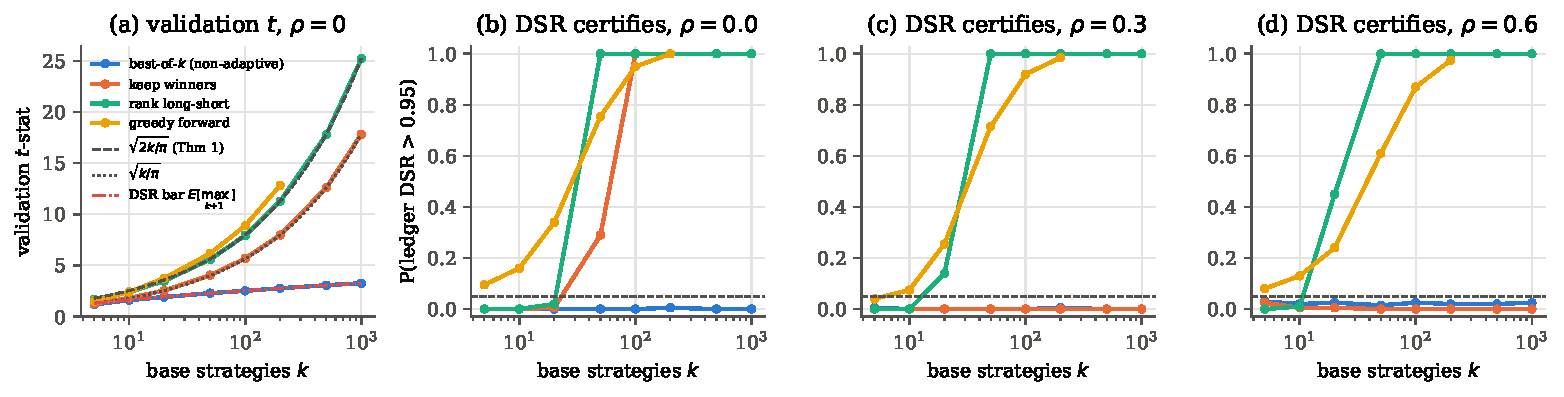
\includegraphics[width=\linewidth]{../figures/fig1_attack.pdf}
\caption{\textbf{E1.} (a) Mean validation $t$ of each analyst on pure noise. The dashed curves are Theorem~\ref{thm:attack}'s predictions and the red dash-dot curve is the DSR bar. (b--d) Probability that ledger DSR $>0.95$ certifies the reported strategy; the dashed line is the nominal 5\%. Out-of-sample $t$-statistics of all certified strategies average zero (Table~\ref{tab:e1} in the appendix).}
\label{fig:attack}
\end{figure}

\subsection{E2: Validity and power of feedback channels}
There are $k=100$ base strategies. In the training regime $m=10$ carry true annualised Sharpe $\mu\in\{0,0.2,0.4,0.6\}$; in the holdout and test regime $m=10$ do, of which a fraction $\phi\in\{1,0.5,0\}$ overlap the training set ($\phi=0$ means the signals rotate completely). There are 500 replicates per cell. The channels are:
\begin{itemize}[leftmargin=*,itemsep=1pt]
\item \emph{greedy+DSR} and \emph{top-$j$+DSR}: the status quo, with full-precision holdout feedback and ledger DSR;
\item \emph{train vault}: choose an equal-weight top-$j$ portfolio ($j\in\{1,2,5,10,15,20\}$) on train, then test once on the holdout at $t>z_{0.95}$;
\item \emph{split vault}: the same with the holdout halved;
\item \emph{verdict} (ours): sealed PASS/FAIL over the six train-ranked candidates ($K=6$);
\item \emph{verdict, adaptive} (stress test): sealed PASS/FAIL with $K=200$. After the six candidates, the analyst perturbs its incumbent on every FAIL (adding or flipping one random signal, and keeping changes that improve the training Sharpe);
\item \emph{split + verdict}: top-$j$ search with full-precision feedback on holdout half A, then a sealed verdict on half B;
\item \emph{greedy + Thresholdout}: greedy search on Thresholdout feedback \citep{dwork2015science} (threshold and noise of 2 and 0.5 SR standard errors, budget 50), certified at $t>z_{0.95}$ on the holdout;
\item \emph{greedy + span bound}: the status-quo greedy report certified at the Scheff\'e/GRS bar of Proposition~\ref{prop:span};
\item \emph{ladder}: a bit-ladder with budget $B=3$ \citep{blum2015ladder}, certified with Corollary~\ref{cor:instances}(iii).
\end{itemize}

\begin{table}[t]\centering\small
\caption{\textbf{E2.} Probability of certification (500 replicates per cell). Column 1 is the null, where the rate is the false-certification rate and the target is $\le0.05$. The other columns give power at annualised signal Sharpe $\mu$ and train/holdout overlap $\phi$.}\label{tab:e2}
\begin{tabular}{l c ccc ccc}\toprule
 & null & \multicolumn{3}{c}{$\mu=0.4$} & \multicolumn{3}{c}{$\mu=0.6$}\\\cmidrule(lr){3-5}\cmidrule(lr){6-8}
channel & & $\phi{=}1$ & $0.5$ & $0$ & $\phi{=}1$ & $0.5$ & $0$\\\midrule
greedy + ledger DSR & \textcolor{red!70!black}{0.97} & 0.98 & 0.99 & 0.98 & 0.99 & 0.99 & 0.99\\
top-$j$ + ledger DSR & \textcolor{red!70!black}{0.95} & 1.00 & 1.00 & 1.00 & 1.00 & 1.00 & 1.00\\
greedy + Thresholdout feedback & \textcolor{red!70!black}{0.29} & 0.45 & 0.37 & 0.35 & 0.68 & 0.49 & 0.36\\
\midrule
greedy + span bound & 0.00 & 0.00 & 0.00 & 0.01 & 0.05 & 0.05 & 0.05\\
train vault & 0.06 & 0.53 & 0.28 & 0.12 & 0.94 & 0.63 & 0.16\\
split vault & 0.06 & 0.28 & 0.24 & 0.24 & 0.60 & 0.58 & 0.59\\
\textbf{sealed verdict} ($K=6$) & 0.03 & 0.47 & 0.21 & 0.06 & 0.95 & 0.56 & 0.08\\
\textbf{sealed verdict}, adaptive ($K=200$) & 0.01 & 0.21 & 0.08 & 0.01 & 0.82 & 0.33 & 0.04\\
\textbf{split + sealed verdict} & 0.03 & 0.23 & 0.18 & 0.20 & 0.48 & 0.54 & 0.54\\
bit-ladder ($B=3$) & 0.00 & 0.01 & 0.01 & 0.01 & 0.06 & 0.05 & 0.04\\
\bottomrule\end{tabular}\end{table}


Table~\ref{tab:e2} and Figure~\ref{fig:channels} show five findings. (1) Under the null, the query-counted DSR channels certify noise in 95--97\% of replicates. Thresholdout \emph{feedback} alone does not prevent this: certifying its greedy report at the usual bar is wrong 29\% of the time, because information still leaks and is not paid for at certification. (2) Every channel with a matching certificate is valid: the sealed verdict at 3.0\%, its adaptive stress test at 0.8\%, split + verdict at 2.6\%, and the vaults at 5.6--6.4\% (binomial s.e.\ 1.1\%). (3) Under stationarity the $K=6$ verdict matches the train vault (power 0.95 vs.\ 0.94 at $\mu=0.6$). Allowing 200 adaptive queries costs some power (0.82) through the higher bar, but buys validity for an analyst that is free to iterate. (4) Under full rotation, channels that search on the training period lose almost all power (verdict 0.08, train vault 0.16). Channels that learn from half of the holdout retain it (split vault 0.59, split + verdict 0.54). Sealing guarantees validity, not power; when the regime may have shifted, the sealed verdict should be applied to the second half of a split holdout. (5) The span bound is valid but powerless (at most 0.05), as Proposition~\ref{prop:span} predicts, and so is the bit-ladder. We report these negative results because they show that \emph{which} bits are revealed matters as much as how many.

\begin{figure}[t]
\centering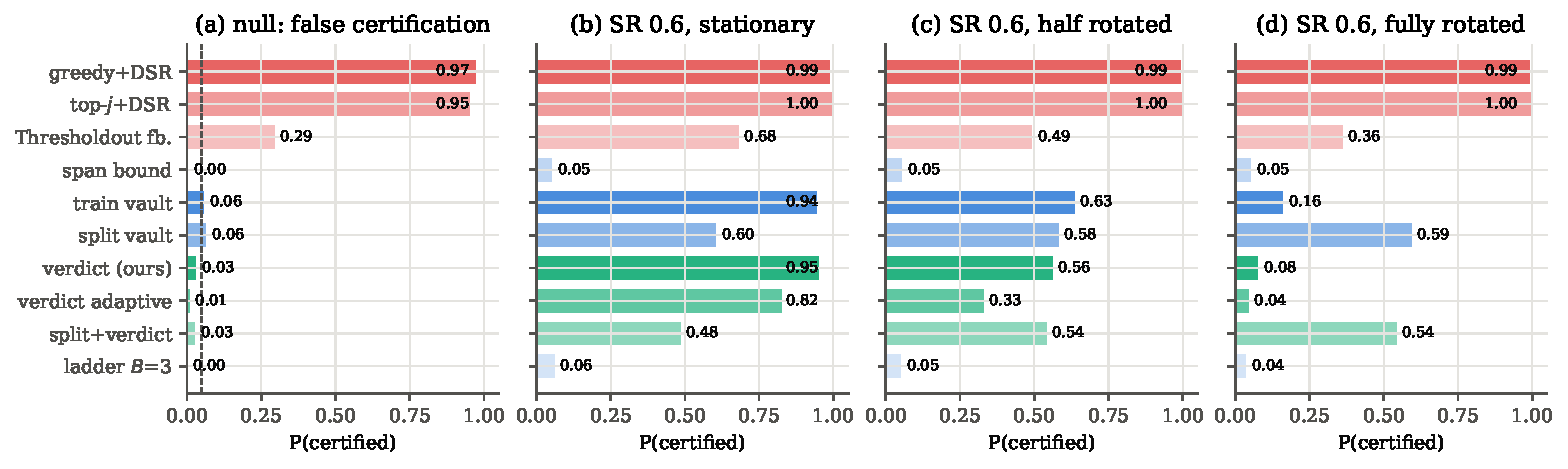
\includegraphics[width=\linewidth]{../figures/fig2_channels.pdf}
\caption{\textbf{E2.} Certification rates by channel. (a) False certification under the null. (b--d) Power when true signals have annualised Sharpe 0.6, as the holdout regime rotates away from training.}
\label{fig:channels}
\end{figure}

\subsection{E3: Real industry strategies, 1970--2026}
We build $k=423$ daily base strategies from the 49 value-weighted Ken French industry portfolios \citep{french2026data} (47 with complete history). Each trades an industry hedged against the market with time-series momentum ($L\in\{5,21,63,126,252\}$ days) \citep{moskowitz2012tsmom}, moving-average crossovers ($\{(5,21),(21,63),(50,200)\}$), or a constant hedged long position. Positions use information up to $t-1$. The splits are train 1970--1999, validation 2000--2012 (the holdout) and test 2013--2026. The mean absolute pairwise correlation is $0.06$. We report (a) one run on actual data and (b) 300 null replicates in which every strategy is demeaned within each split and time is jointly resampled with a stationary bootstrap \citep{politis1994stationary} (mean block 21 days), which preserves cross-correlation, volatility clustering and fat tails while removing all true edge.

\begin{table}[t]\centering\small
\caption{\textbf{E3.} 423 real hedged industry strategies. Null: false-certification rate over 300 stationary-bootstrap replicates (binomial s.e.\ in parentheses). Actual: validation (2000--2012) and test (2013--2026) $t$ of the reported strategy, and whether it was certified.}\label{tab:e3}
\begin{tabular}{l c ccc}\toprule
 & null & \multicolumn{3}{c}{actual data}\\\cmidrule(lr){3-5}
workflow & P(certify) & val.\ $t$ & test $t$ & certified\\\midrule
greedy + ledger DSR & 1.000 (0.000) & 15.23 & -0.76 & yes\\
rank long--short + ledger DSR & 1.000 (0.000) & 9.96 & -0.02 & yes\\
sign flip + ledger DSR & 1.000 (0.000) & 8.32 & +0.51 & yes\\
top-$j$ + ledger DSR & 0.837 (0.021) & 7.06 & +0.53 & yes\\
\midrule
greedy + span bound & 0.000 (0.000) & 15.23 & -0.76 & no\\
train vault & 0.037 (0.011) & 0.38 & +0.02 & no\\
\textbf{sealed verdict} & 0.013 (0.007) & 0.38 & +0.02 & no\\
\textbf{split + sealed verdict} & 0.027 (0.009) & 5.81 & +0.75 & no\\
\bottomrule\end{tabular}\end{table}


On the null, every adaptive status-quo workflow is DSR-certified in 84--100\% of replicates. The span bound certifies nothing (its bar is $t>23.4$), and the train vault (3.7\%), the sealed verdict (1.3\%) and split + verdict (2.7\%) are valid (Figure~\ref{fig:real}a). On actual data (Figure~\ref{fig:real}b) all four status-quo workflows earn DSR $=1.00$ with validation $t$ between 7.1 and 15.2 and then deliver test $t$ between $-0.8$ and $0.5$ over 2013--2026. The honest channels decline to certify; the training-period winners did not persist into the 2000s. A single historical path cannot separate overfitting from genuine post-2000 decay of these signals, so we treat panel~(b) as illustrative. The validity claims rest on the 300 null replicates in panel~(a), where any certification is false by construction.

\begin{figure}[t]
\centering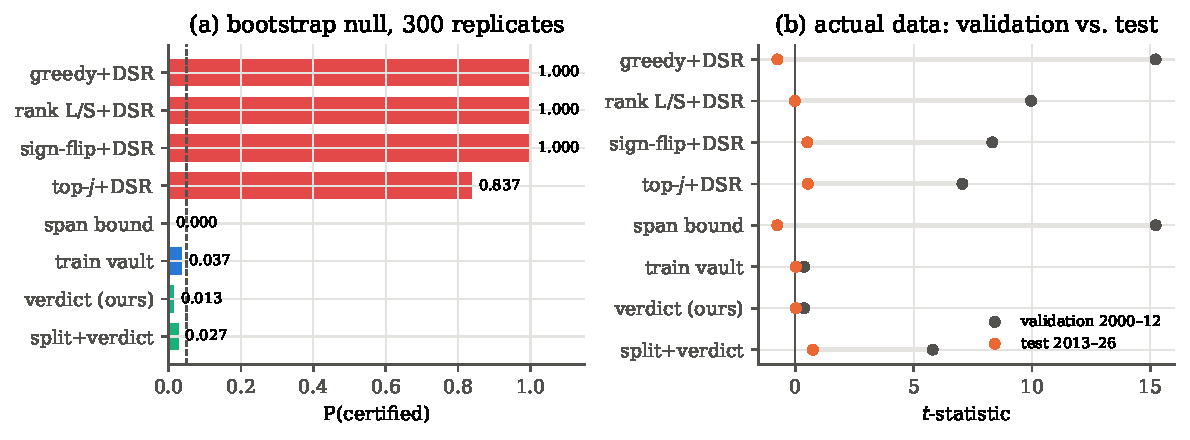
\includegraphics[width=0.92\linewidth]{../figures/fig3_real.pdf}
\caption{\textbf{E3.} (a) False certification on 300 stationary-bootstrap null replicates of the 423 real strategies. (b) Actual data: validation (2000--2012) versus test (2013--2026) $t$-statistics of each workflow's reported strategy.}
\label{fig:real}
\end{figure}

\subsection{E4 (exploratory): LLM research agents}
We place open-weight instruction models, Qwen2.5-7B and Qwen2.5-72B \citep{qwen2024qwen25} served with vLLM, in the research loop over the 423 real strategies. Each turn the agent writes one sentence of reasoning and a JSON portfolio of up to 20 signals. It receives its training-period Sharpe (1970--1999) and either the validation Sharpe (status quo) or a sealed verdict. Each condition runs 8 episodes on actual data and 24 on null data. Every null episode uses its own bootstrap replicate, so its data are synthetic and pretraining knowledge of market history cannot help. We also give the 72B agent a \emph{batch tool} that evaluates up to 20 portfolios per turn for 15 turns, mimicking code-executing agents that run backtest sweeps. The status-quo report is the best-validation proposal, certified by ledger DSR over the \emph{distinct} proposals (duplicates are counted once, the convention used throughout).

\begin{table}[t]\centering\small
\caption{\textbf{E4.} LLM research agents (40 turns of one proposal, or 15 turns of up to 20 proposals with the batch tool; ``queries'' is the mean number of holdout queries actually made). Null rows: each episode uses its own bootstrap-null replicate, so every certification is false. Naive channel: report the best-validation proposal, certified by ledger DSR$>0.95$. Verdict channel: sealed PASS/FAIL with budget $K$ equal to the query allowance. Means over episodes.}\label{tab:e4}
\begin{tabular}{ll l cc ccc}\toprule
agent & data & channel & episodes & queries (distinct) & P(certify) & val.\ $t$ & test $t$\\\midrule
Qwen2.5-7B & actual & full Sharpe + DSR & 8 & 40 (22) & 0.000 & 1.99 & +0.33\\
Qwen2.5-7B & actual & sealed verdict & 8 & 39 (21) & 0.000 & -0.11 & -0.82\\
Qwen2.5-7B & null & full Sharpe + DSR & 24 & 39 (19) & 0.042 & 1.17 & +0.27\\
Qwen2.5-7B & null & sealed verdict & 24 & 38 (24) & 0.000 & -0.21 & +0.03\\
\midrule
Qwen2.5-72B & actual & full Sharpe + DSR & 8 & 40 (29) & 0.000 & 1.58 & +0.15\\
Qwen2.5-72B & actual & sealed verdict & 8 & 40 (29) & 0.000 & 0.72 & +0.08\\
Qwen2.5-72B & null & full Sharpe + DSR & 24 & 40 (30) & 0.042 & 1.21 & +0.09\\
Qwen2.5-72B & null & sealed verdict & 24 & 31 (26) & 0.000 & 0.02 & +0.01\\
\midrule
72B + batch tool & actual & full Sharpe + DSR & 8 & 63 (36) & 0.125 & 2.32 & -0.39\\
72B + batch tool & actual & sealed verdict & 8 & 53 (44) & 0.000 & 0.37 & +0.27\\
72B + batch tool & null & full Sharpe + DSR & 24 & 93 (35) & 0.000 & 1.77 & +0.16\\
72B + batch tool & null & sealed verdict & 24 & 76 (62) & 0.000 & 0.15 & +0.19\\
\bottomrule\end{tabular}\end{table}


Table~\ref{tab:e4} and Figure~\ref{fig:agents} give a more nuanced picture than Theorem~\ref{thm:attack} alone. Qualitatively, the 72B agent does exactly what the theory describes. With the batch tool it writes, for example, \emph{``The combination of hold\_Aero and tsmom\_Aero\_63 shows the highest validation Sharpe. Testing further variations and adding other promising signals''}, and it grows an ensemble of validation winners turn by turn, which is greedy forward selection on the holdout. Quantitatively, today's agents are \emph{inefficient} adaptive analysts. The single-proposal agents converge within about 15 turns: the 7B model makes 19--22 distinct proposals in 40 turns and the 72B model 29--30, after which they resubmit near-identical portfolios. The batch agent uses its full 15 turns but submits only about 6 portfolios per turn rather than the 20 allowed, a median of about 70 queries (35 distinct) on the null. Their best null validation $t$ plateaus at 1.2--1.8, whereas the scripted greedy analyst of E1 reaches $t\approx4$--$6$ with a comparable number of queries (40--100). Ledger DSR therefore certified only 2 of 72 null status-quo episodes (2.8\%, both from single-proposal agents), within the nominal 5\%. Neither certification is driven by adaptivity. Both have validation $t$ ($2.64$ and $2.99$) at the Bonferroni bar for their number of distinct proposals, and are certified because highly correlated proposals shrink DSR's scale estimate ($nV=0.37$ and $0.11$). This is a second, non-adaptive weakness of ledger DSR (Corollary~\ref{cor:instances}(i)). On actual data one batch episode is certified (validation $t=3.30$, DSR $0.99$, $nV=0.21$) and then has test $t=-0.63$ over 2013--2026.

The honest reading is that \emph{chat-style} LLM agents do not yet exploit a holdout within a single session. The adaptive capacity is there for any agent that searches more efficiently, for example by writing code, running for longer, or being trained to search. The sealed verdict made no false certifications in any condition and costs nothing in these settings.

\begin{figure}[t]
\centering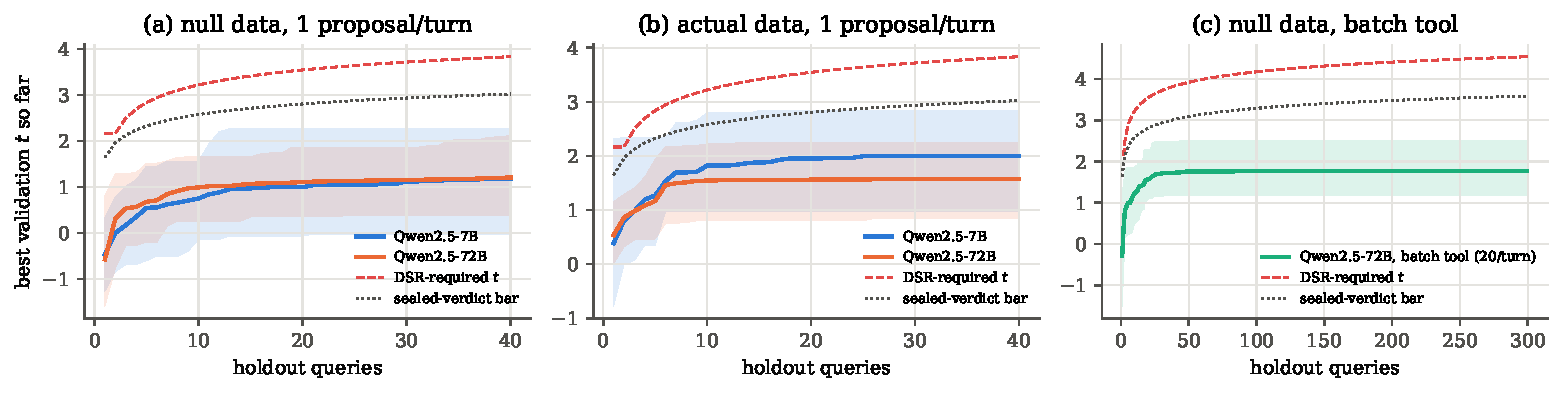
\includegraphics[width=\linewidth]{../figures/fig4_agents.pdf}
\caption{\textbf{E4.} Best validation $t$ found so far by LLM agents under the full-Sharpe channel (mean and 10--90\% band over episodes), against the $t$ that ledger DSR requires and the sealed-verdict bar for the same number of queries.}
\label{fig:agents}
\end{figure}

\subsection{E5 (exploratory): RL alpha mining with GRPO}
RL alpha miners optimise a backtest metric directly \citep{yu2023alphagen}, which makes them the most aggressive adaptive analysts in practice. We fine-tune Qwen2.5-1.5B-Instruct with GRPO \citep{shao2024deepseekmath} (LoRA rank 32, learning rate $5\times10^{-5}$, 300 steps $\times$ 32 completions $=9{,}600$ scored portfolios). The policy emits one JSON portfolio per completion, and invalid outputs receive $-1$. We compare three rewards: the portfolio's validation Sharpe (\emph{val}); its training Sharpe with the holdout sealed (\emph{train}); and an AlphaGen-style \emph{pool} reward, the marginal improvement in validation Sharpe of a growing combined portfolio, into which the batch's best improver is merged each step \citep{yu2023alphagen}. The pool reward is the RL analogue of Theorem~\ref{thm:attack}.

\begin{table}[t]\centering\small
\caption{\textbf{E5.} GRPO on Qwen2.5-1.5B, 300 steps $\times$ 32 completions; s2 and s3 are additional seeds (fresh null replicate and RL seed). Reported strategy: the best distinct portfolio by the reward split. Validation-reward runs are certified by ledger DSR over all distinct portfolios; the pool run reports the final pool, with the ledger comprising all distinct portfolios and pool states; train-reward runs by the sealed verdict over the 40 best-by-train portfolios.}\label{tab:e5}
\begin{tabular}{ll ccc cc}\toprule
data & reward & distinct portfolios & val.\ $t$ & test $t$ & DSR & certified\\\midrule
null & validation & 200 & 3.87 & +0.40 & 0.680 & no\\
null & validation (s2) & 2450 & 2.48 & +0.28 & 0.522 & no\\
null & validation (s3) & 364 & 2.34 & -0.61 & 0.339 & no\\
null & train (sealed) & 106 & -0.57 & -0.22 & -- & no\\
null & validation pool & 300 & 4.12 & +0.74 & 0.763 & no\\
null & validation pool (s2) & 202 & 2.86 & -0.38 & 0.695 & no\\
null & validation pool (s3) & 9201 & 12.01 & -0.56 & 1.000 & yes\\
actual & validation & 1409 & 5.00 & -0.26 & 0.948 & no\\
actual & train (sealed) & 3151 & 0.10 & +0.13 & -- & no\\
\bottomrule\end{tabular}\end{table}


Table~\ref{tab:e5} and Figure~\ref{fig:grpo} show that, in every run (one seed per arm), the RL miner overfits the split it is rewarded on. With validation reward on the null, the policy finds a portfolio with validation $t=3.87$ within about 10 steps and collapses onto it (test $t=+0.40$). On actual data the mean validation Sharpe of its samples rises for about 120 steps. The best portfolio, first generated at step 187, has validation $t=5.00$ (a 2000--2012 annualised Sharpe of 1.39) and then \emph{loses money} over 2013--2026 (test $t=-0.26$). Ledger DSR over the 1,409 distinct portfolios it evaluated gives $0.948$: DSR declines to certify, but by a margin of $0.002$. The pool reward produces a combined portfolio with validation $t=4.12$ within 21 steps (DSR $0.763$ over all distinct portfolios and pool states). The pool, however, is not the many-signal noise ensemble of Theorem~\ref{thm:attack}. Six of its seven signals are variants of a single industry (Aero), so the policy has found one spurious industry and re-weighted it. It then loses entropy and stops proposing improvers, and the pool does not change after step 21.

With training reward and the holdout sealed, the RL miner overfits the \emph{training} period instead. On actual data it converges to a basket of 5- and 21-day industry momentum signals with a 1970--1999 annualised Sharpe of 4.3, consistent with the strong short-horizon autocorrelation of pre-2000 daily industry returns. Its validation and test Sharpe are about zero. The sealed verdict over the 40 best-by-training portfolios correctly certifies nothing in either train-reward run.

As with LLM agents, the RL policies substantially inflate validation performance relative to test performance, but GRPO's mode collapse caps how many distinct holdout queries they effectively make (106--3,151 distinct portfolios out of 9,600 completions). In this configuration ledger DSR is not defeated, although in one run its margin is $0.002$. The sealed reward makes validity independent of such optimiser details.


\begin{figure}[t]
\centering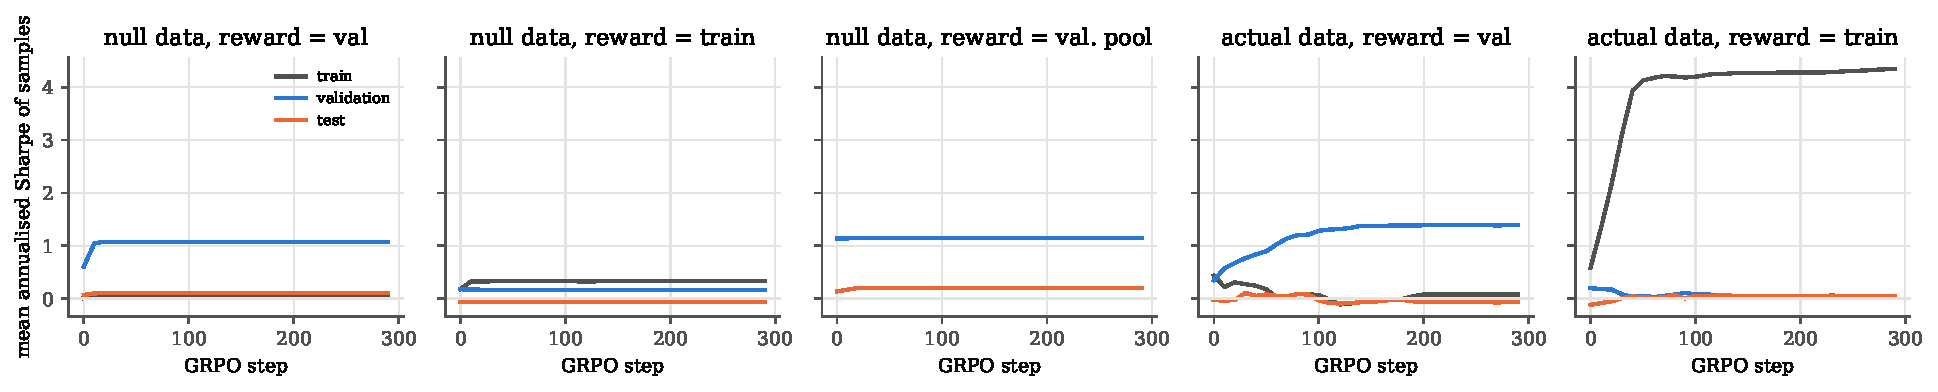
\includegraphics[width=\linewidth]{../figures/fig5_grpo.pdf}
\caption{\textbf{E5.} Mean annualised Sharpe of sampled portfolios on the training, validation and test splits during GRPO training (10-step bins).}
\label{fig:grpo}
\end{figure}


%======================================================================
\section{Related work}
%======================================================================
\paragraph{Backtest overfitting.} Data snooping in finance has been studied since \citet{lo1990data}. Corrections include reality checks and step-wise tests \citep{white2000reality,hansen2005spa,romano2005stepwise,sullivan1999data}, multiple-testing haircuts \citep{harvey2016cross}, the DSR and PBO \citep{bailey2014deflated,bailey2017pbo}, and practice guides \citep{lopezdeprado2018advances}. All of these take the candidate family as fixed. \citet{gelman2014garden}'s ``garden of forking paths'' names the adaptive problem informally; we quantify it for Sharpe ratios.

\paragraph{Adaptive data analysis.} Differential-privacy-based reusable holdouts \citep{dwork2015science,dwork2015generalization,bassily2016algorithmic}, lower bounds \citep{hardt2014preventing}, information-theoretic bias bounds \citep{russo2016controlling,xu2017information}, and the Ladder for leaderboards \citep{blum2015ladder} are the foundations we specialise. \citet{freedman1983note} showed that screening regressors and refitting produces spurious significance; Theorem~\ref{thm:attack} is its strategy-ensemble analogue with an exact rate and an explicit DSR comparison.

\paragraph{LLM and RL alpha discovery.} RL formula miners optimise validation-style metrics \citep{yu2023alphagen}, and LLM-driven search systems iterate on backtests \citep{shi2025alphaforge}. \citet{gencay2026honest} add a trial ledger and DSR, which our results show is insufficient under adaptivity. \citet{qu2026propose} achieve anytime validity on live data with e-processes, which is complementary: our certificate works on historical holdouts and needs no waiting. Validation-reward overoptimisation in RL mirrors reward-model overoptimisation \citep{gao2023scaling}.

%======================================================================
\section{Limitations}
%======================================================================
(1) Theorems~\ref{thm:attack} and~\ref{thm:transcript} are stated for i.i.d.\ periods. Serial dependence changes constants (one can use HAC $t$-statistics) but not rates. (2) Theorem~\ref{thm:transcript} is a worst-case union bound and is conservative for cooperative analysts. (3) Sealing cannot fix look-ahead leakage through pretrained weights (Section~\ref{sec:sealed}); our validity claims rest on synthetic and bootstrap nulls. (4) The verdict channel has no power advantage over a one-shot vault in a single episode. Its value is that it remains valid while an agent iterates, which a vault does not. (5) Our real universe is one asset class with simple signals; richer universes raise $k$ and strengthen the attack. (6) The agent experiments use open-weight models up to 72B parameters with a 32k-token context, and the RL policies (1.5B, LoRA, no entropy bonus) collapse onto a few portfolios within tens of steps. Frontier agents with code execution, longer memory, or RL with diversity incentives would search more efficiently. Our results bound current behaviour; they do not forecast it. (7) E5 uses one seed per arm, and its null arms share a single bootstrap replicate (also used by E4's seed-0 episodes); E4 has 8 actual-data episodes per arm. (8) Industries are hedged with a unit beta, and the 47-industry universe is selected by full-sample data availability.

%======================================================================
\section{Conclusion}
%======================================================================
When the researcher is adaptive, whether a person, a script or an agent, counting trials does not measure overfitting. Counting \emph{bits} does. Ordinary workflows such as keeping the validation top-$j$ already defeat complete-ledger DSR on pure noise. Today's LLM agents and small RL miners behave in the same way but, at current scale, search too inefficiently to do so; that margin is a property of today's agents, not of the method. A holdout that only says PASS or FAIL can be reused by any agent with a bar no harsher than DSR's. A holdout that prints Sharpe ratios can be corrected only by a span bound that pays for the full dimension of the strategy space. We recommend that agentic research frameworks expose holdouts only through sealed, budgeted verdicts, and that published agentic backtests report the channel through which the agent saw the holdout, not just the number of trials.

\paragraph{Code and data availability.} All code, raw results (including every LLM transcript and RL ledger) and the data pipeline are available at \url{https://github.com/shloksobti/deflate-by-bits}. Return data are from the Ken French Data Library (CRSP 2026-08 vintage).

\paragraph{Acknowledgments.} The analysis, experiments, code and drafting of this paper were carried out with substantial assistance from an AI system (Claude, Anthropic), including an AI-conducted adversarial review. The author directed the work and takes full responsibility for its content.

\bibliographystyle{plainnat}
\bibliography{refs}

\appendix
\section{Proofs}\label{app:proofs}
\paragraph{Proof of Theorem~\ref{thm:attack}.}
Let $\bar r=\frac1n\sum_t r_t$ and $\hat\Sigma$ the sample covariance. Then $Z_i=\sqrt n\,\bar r_i/\hat\sigma_i$, and by the CLT and $\hat\Sigma\to\Sigma$ a.s., $\sqrt n\,\bar r\Rightarrow\mathcal N(0,\Sigma)$, so $Z\Rightarrow Z^\ast\sim\mathcal N(0,\Sigma)$. Represent $Z^\ast=\sqrt\rho F\mathbf 1+\sqrt{1-\rho}\,\varepsilon$ with $F\sim\mathcal N(0,1)$ and $\varepsilon\sim\mathcal N(0,I_k)$ independent. Because $\operatorname{med}(Z^\ast)=\sqrt\rho F+\sqrt{1-\rho}\operatorname{med}(\varepsilon)$, the sign vector $s(Z^\ast)=\operatorname{sign}(\varepsilon-\operatorname{med}\varepsilon)$ is free of $F$. For even $k$ (ties have probability zero) exactly $k/2$ entries are $+1$, so $\mathbf 1^\top s=0$.

The reported portfolio $\hat w=s/k$ has $\sqrt n\,\hat w^\top\bar r=\frac1k s^\top(\sqrt n\,\bar r)$ and sample variance $\hat w^\top\hat\Sigma\hat w$. The map $x\mapsto s(x)$ is continuous at $Z^\ast$ almost surely, so by the continuous-mapping theorem and $\hat\Sigma\to\Sigma$,
\[
\tH(\hat w)=\frac{\frac1k s^\top\sqrt n\,\bar r}{\sqrt{\hat w^\top\hat\Sigma\hat w}}\;\Rightarrow\;\frac{\frac1k s^\top Z^\ast\cdot\sigma}{\sqrt{s^\top\Sigma s}/k},
\]
where we used $\sqrt n\,\bar r=\operatorname{diag}(\hat\sigma)Z$ with $\hat\sigma_i\to\sigma=1$. Now $s^\top\Sigma s=(1-\rho)\|s\|^2+\rho(\mathbf 1^\top s)^2=(1-\rho)k$ and $s^\top Z^\ast=\sqrt{1-\rho}\,s^\top\varepsilon=\sqrt{1-\rho}\sum_i|\varepsilon_i-\operatorname{med}\varepsilon|$, using $s^\top\mathbf 1\operatorname{med}\varepsilon=0$. Hence $\tH(\hat w)\Rightarrow k^{-1/2}\sum_i|\varepsilon_i-\operatorname{med}\varepsilon|$. Finally $\operatorname{med}\varepsilon\to0$ a.s.\ and $\frac1k\sum_i|\varepsilon_i-m|$ is $1$-Lipschitz in $m$, so $\frac1k\sum_i|\varepsilon_i-\operatorname{med}\varepsilon|\to\E|\varepsilon_1|=\sqrt{2/\pi}$ a.s., which gives $\tH(\hat w)/\sqrt{2k/\pi}\to1$.

For $\rho=0$ and $s_i=\operatorname{sign}(Z_i)$ the same argument gives $s^\top\Sigma s=k$ and $s^\top Z^\ast=\sum|\varepsilon_i|$, with the same limit. For keep-winners, $\hat w=\mathbf{1}\{Z>0\}/|S|$ with $|S|/k\to1/2$, mean $\sum_{i\in S}\varepsilon_i/|S|$ and variance $1/|S|$. The limit is $|S|^{-1/2}\sum_{i\in S}\varepsilon_i\approx\sqrt{k/2}\,\E[\varepsilon\mid\varepsilon>0]=\sqrt{k/2}\sqrt{2/\pi}=\sqrt{k/\pi}$. \qed

\paragraph{Proof of Corollary~\ref{cor:dsr}.}
The ledger's per-period Sharpe estimates are $Z_i/\sqrt n$ for $i\le k$ together with $\tH(\hat w)/\sqrt n$. Their sample variance satisfies $nV=\frac1{k}\big[\sum_i(Z_i-\bar Z)^2+(\tH(\hat w)-\bar Z)^2\big](1+o(1))$. The first term tends to $(1-\rho)$ (the cross-sectional variance of $Z^\ast$ given $F$) and the second to $(2k/\pi)/k=2/\pi$. With Gaussian returns $\hat\gamma_3\to0$ and $\hat\gamma_4\to3$, so the denominator of~\eqref{eq:dsr} tends to $\sqrt{1+\SR^2/2}=1+O(k/n)$. The numerator is $\sqrt{n-1}(\SR-\SR_0)=\tH(\hat w)-\sqrt{nV}\,\E\max_{k+1}+o(1)$, and $\E\max_{k+1}\le\sqrt{2\ln(k+1)}$. Therefore the DSR $z$-score is at least $\sqrt{2k/\pi}(1+o_p(1))-\sqrt{1-\rho+2/\pi}\sqrt{2\ln(k+1)}\to\infty$ in probability. \qed

\paragraph{Proof of Proposition~\ref{prop:tight}.}
A channel revealing $b$ bits has $|\cT|\le2^b$. By Theorem~\ref{thm:transcript} and the Gaussian tail $\bar\Phi^{-1}(p)=\sqrt{2\ln(1/p)}(1+o(1))$ as $p\to0$, the bar is $\sqrt{2(b\ln2+\ln(1/\alpha))}(1+o(1))=\sqrt{2b\ln 2}(1+o(1))$. The sign-flip analyst's report depends on $H$ only through $(\operatorname{sign}Z_i)_{i\le k}$, which is $k$ bits, and by Theorem~\ref{thm:attack} its $t$ is $\sqrt{2k/\pi}(1+o_p(1))$. Hence, for $b=o(n)$ and in the sequential limit of Theorem~\ref{thm:attack}, the supremum over $b$-bit analysts of the null $(1-\alpha)$-quantile of $\tH(\hat w)$ lies between $0.80\sqrt b$ and $1.18\sqrt b$. \qed

\paragraph{Proof of Proposition~\ref{prop:span}.} For any $w$ in the span, Cauchy--Schwarz in the $\hat\Sigma$ inner product gives $n(w^\top\bar r)^2/(w^\top\hat\Sigma w)\le n\,\bar r^\top\hat\Sigma^{-1}\bar r$. Under Gaussian $H_0$ the right-hand side is Hotelling's $T^2$, distributed as $\frac{k(n-1)}{n-k}F_{k,n-k}$ \citep{scheffe1953method,gibbons1989test}. The bound holds simultaneously for every $w$, hence for any data-dependent report. \qed

\paragraph{Remark (serial dependence and non-Gaussian rows).} With stationary, weakly dependent returns, Theorem~\ref{thm:attack} holds with $\Sigma$ replaced by the long-run covariance and a HAC $t$-statistic. Theorem~\ref{thm:transcript} needs the tail of the null $t$-statistic to be controlled at level $\alpha/|\cT|$. For i.i.d.\ non-Gaussian rows this follows from self-normalised moderate-deviation results when $c_\cT=o(n^{1/6})$ and the third moment is finite. For HAC statistics tail accuracy is poorer, and a block-bootstrap calibration of $\bar G$ is advisable when $|\cT|$ is large.


\section{Additional tables}
\begin{table}[h]\centering\small
\caption{E1 details ($\rho=0$, 200 replicates): mean validation $t$ / mean test $t$ / P(ledger DSR$>0.95$).}\label{tab:e1}
\begin{tabular}{lcccc}\toprule
analyst & $k=10$ & $k=50$ & $k=100$ & $k=1000$\\\midrule
best-of-$k$ & 1.6 / -0.10 / 0.00 & 2.3 / -0.03 / 0.00 & 2.5 / -0.06 / 0.00 & 3.2 / -0.01 / 0.00\\
keep winners & 1.8 / +0.05 / 0.00 & 4.0 / +0.02 / 0.29 & 5.7 / +0.05 / 1.00 & 17.8 / -0.03 / 1.00\\
sign flip & 2.6 / -0.02 / 0.00 & 5.7 / -0.06 / 1.00 & 8.0 / -0.08 / 1.00 & 25.2 / -0.00 / 1.00\\
rank long--short & 2.4 / -0.02 / 0.00 & 5.6 / -0.09 / 1.00 & 7.9 / -0.06 / 1.00 & 25.2 / -0.01 / 1.00\\
greedy forward & 2.4 / -0.02 / 0.16 & 6.2 / +0.05 / 0.76 & 8.9 / -0.01 / 0.95 & --\\
\bottomrule\end{tabular}\end{table}


\end{document}
